
\documentclass[5pt,a4paper]{article}
\usepackage{geometry}
\geometry{
	a4paper,
	total={170mm,257mm},
	left=20mm,
	top=20mm,
}
\usepackage[latin1]{inputenc}
\usepackage{amsmath}
\usepackage{amsfonts}
\usepackage{amssymb}
\usepackage{graphicx}
\begin{document}
	\title{Machine learning Homework- Optimisation}
	\author{Abinav Ravi Venkatakrishnan - 03694216 and Abhijeet Parida - 03679676}
	\maketitle
	\section*{Problem 1:}
	\begin{enumerate}
		\item we know that sum of convex function is a convex function. $x^2, 2y,cos(sin(\sqrt{\pi}))$ are convex functions because linear and constant are convex.
		
		$-min\{-x^2,log(y)\}=max\{x^2,-log(y)\}$. The max is convex if both functions are convex which is true for our case. So, it is a convex function.
		
		\item we know that the point-wise addition of two convex function is convex; but here $log(x)$ and $-x^3$ are concave; so overall is concave.
		\item $-min\{log(3x + 1), -x^4 -3x^2 + 8x-42\} =  max\{-log(3x + 1), x^4 +3x^	2 - 8x + 42\}$ The max is convex if both functions are convex which is true for our case. So, it is a convex function.
		
		\item by plotting Fig. \ref{plot}, we see that the function $-x^2y $ is not convex. So, it is not a convex function. 
	\end{enumerate}\
	\begin{figure}[h!]
		\centering
		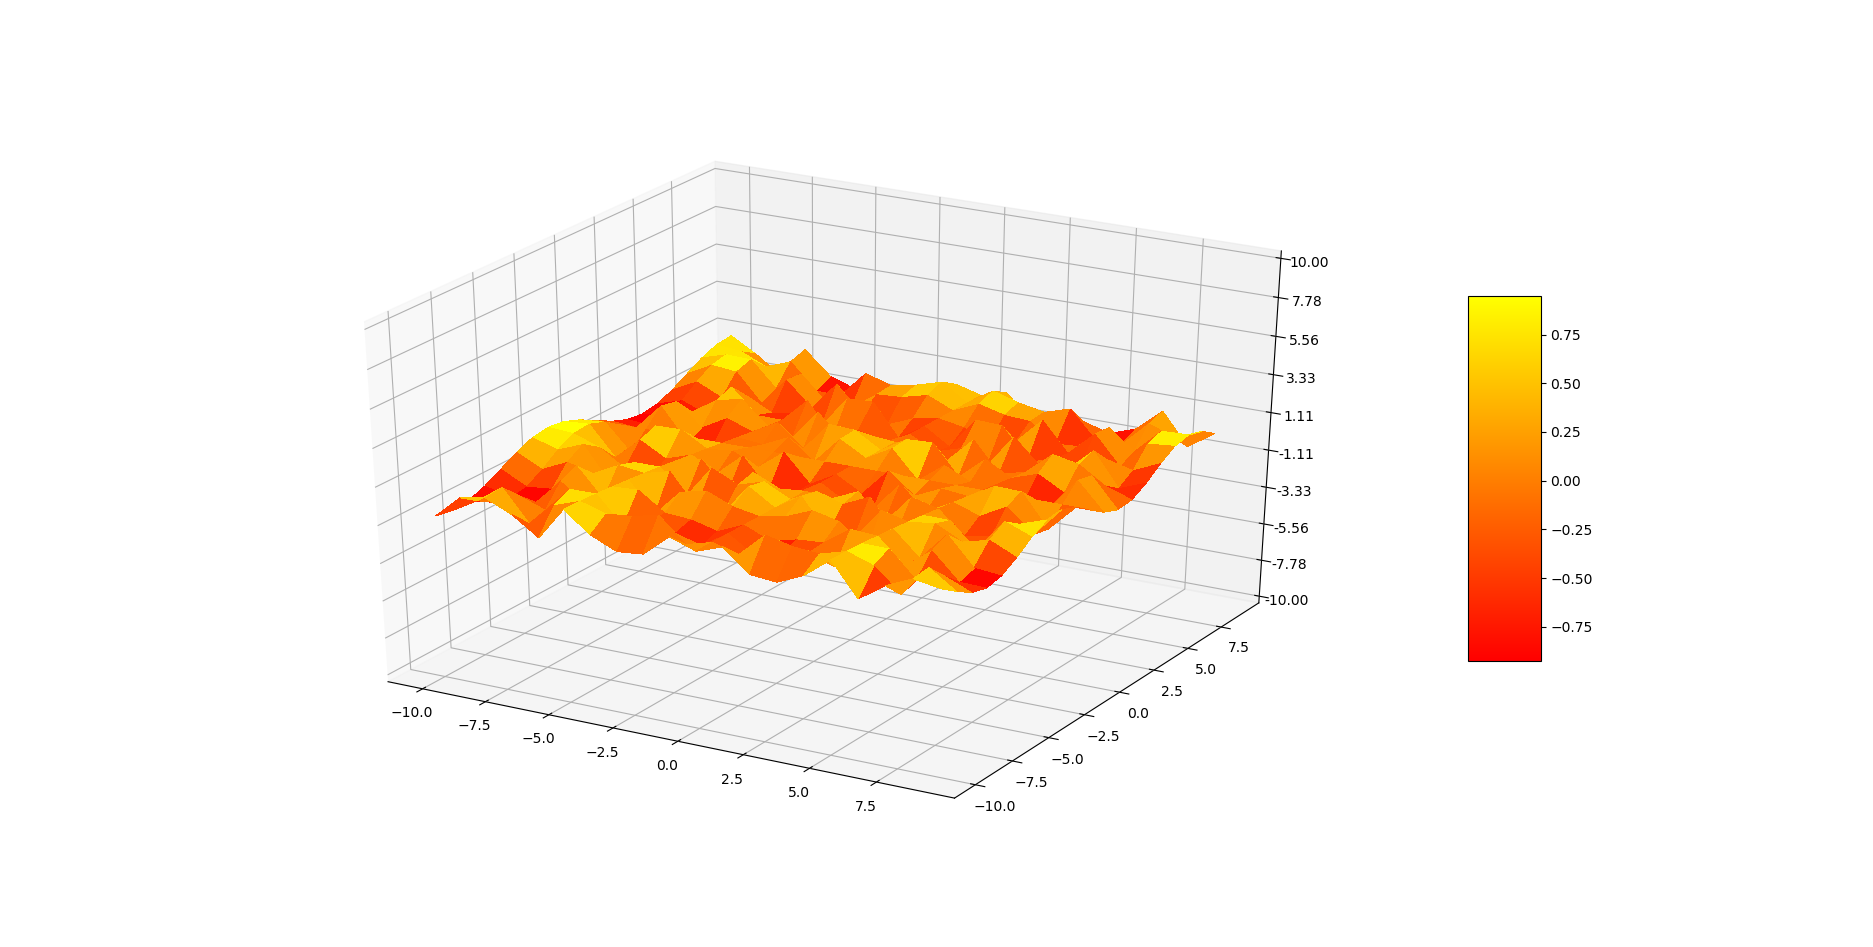
\includegraphics[width=1\textwidth]{x2y.png}
		\caption{}
		\label{plot}
	\end{figure}
	
	\section*{Problem 2:}
	we know that the functions $f_1 \text{and} f_2$ are convex in $\mathcal{R}$.\\
	so,
	\begin{equation}
	\lambda_1 f_1(x_1)+(1-\lambda_1)f_1(x_2) \geqslant f_1(\lambda_1 x_1+(1-\lambda_1)x_2)
	\label{one}
	\end{equation}
	and \\
	\begin{equation}
	\lambda_1 f_2(x_1)+(1-\lambda_1)f_2(x_2) \geqslant f_2(\lambda_1 x_1+(1-\lambda_1)x_2)
	\label{two}
	\end{equation}

	$h(x)=max(f_1(x),f_2(x))$ and given $f_1 \text{and} f_2$ are convex can be written as
	\[\begin{cases}
		f_1(x)&; x \geqslant C\\
		f_2(x)&; x \leqslant C
	\end{cases}
	\]
	
	for $x_1,x_2 \geqslant C$; Eqn \ref{one} is true and for $x_1,x_2 \leqslant C$; Eqn \ref{two} is true.
	
	for the case  $x_2 \geqslant C$ and $x_1 \leqslant C$. We have to show two scenario to be true.
	\begin{equation}
	\lambda_1 f_1(x_1)+(1-\lambda_1)f_2(x_2) \geqslant f_1(\lambda_1 x_1+(1-\lambda_1)x_2)
	\label{one1}
	\end{equation}
	Eq. \ref{one1} is true because Eq. \ref{one} is true and on the LHS $(1-\lambda_1)f_2(x_2) > (1-\lambda_1)f_1(x_2)$ from definition of $h(x)$.
	\begin{equation}
	\lambda_1 f_1(x_1)+(1-\lambda_1)f_2(x_2) \geqslant f_2(\lambda_1 x_1+(1-\lambda_1)x_2)
	\label{two2}
	\end{equation}
	Eq. \ref{two2} is true because Eq. \ref{two} is true and on the LHS $\lambda_1f_1(x_1) > \lambda_1f_2(x_1)$ from definition of $h(x)$.
	\section*{Problem 3:}
	we know that $f_1 \text{and} f_2$ are convex and their exist a minima $x_1 \text{and} x_2$ such that\\
	
	\begin{equation}
		f_1'(x_1)=0 \text{ ; } f_1''(x_1)>0
		\label{eqn1}
	\end{equation}
		\begin{equation}
	f_2'(x_2)=0 \text{ ; } f_2''(x_2)>0
	\label{eqn2}
	\end{equation}
	
	for our function $f_1(f_2(x))$, the local minima can be found at \\
	\begin{equation}
	f_1'(f_2(x)).f_2'(x)=0 
	\label{eqn3}
	\end{equation}
	
	From Eq. \ref{eqn1} and Eq. \ref{eqn2} the possible candidates for minima of $f_1f_2(x)$ is $x=x_2$ and $f_2(x)=x_1$.
	
	For the critical point  $x=x_2$ is minima if $(f_1f_2(x))''>0$
	\begin{equation}
	f_2''(x).f_1'(f_2(x))+f_2'(x).f_1''(f_2(x)).f_2'(x)
	\label{minima}
	\end{equation}
	we know that $f_2'(x_2).f_1''(f_2(x_2)).f_2'(x_2)=0$ from Eq. \ref{eqn2} and in the term $f_2''(x).f_1'(f_2(x))$,$f_2''(x)$ is +ve from Eq. \ref{eqn2}. Therefore, the final sign of the Eq.\ref{minima} depends on the sign of $f_1'(f_2(x))$,$f_2''(x)$. Since it is positive/negative we cannot say it is convex always.\\\\
	
	For the critical point  $f_2(x)=x_1$ is minima if $(f_1f_2(x))''>0$.\\
	we know that $f_2''(x).f_1'(f_2(x))=0$ from Eq. \ref{eqn3} and in the term $f_2'(x).f_1''(f_2(x)).f_2'(x) $,$f_2''(x)$ is  always +ve from Eq. \ref{eqn2}. Therefore, the statement is true in this case.
	
	Overall, the statement is true for some $f_1,f_2$ and not true for other $f_2,f_1$ 

\section*{Problem 4:}Theorem:
Suppose $f:x\mapsto\mathcal{R}$ is a differentiable function
and $\mathcal{R}$ is convex. Then $f$ is convex iff for $x, y \in \mathcal{X}$ then \\
\begin{equation}
	f(y)\geqslant f(x)+(y-x)^T \nabla f(x)
\end{equation}
for $ \nabla f(x)=0$, we get $f(y)\geqslant f(x)$ hence $f(x)$ is the lowest possible value when$ \nabla f(x)=0$

\end{document}